%=============================================================================================================================================================================================
%: (\emph{i}) Low-level Similarity: Computing similarity between app using low-level data, e.g: source code, byte code, function calls, API reference, etc. (\emph{ii}) High-level Similarity: Detecting the semantic similarity using metadata, such as: topic distribution, readme file, description, star events, etc.%This classification is used throughout this paper as a means to distinguish between the approaches with regards to the input information used for similarity computation.
%A pre-processing stage is performed to extract identifiers such as variable names, function names and to remove unrelated factors such as comment. With the application of Latent Semantic Analysis, software is considered as a document and each identifier is considered as a word. LSA is used for extracting and representing the contextual usage meaning of words by statistical computations applied to a large corpus of text. 
%$CLAN$ works based on the document framework for computing similarity, semantic anchors, e.g. those that define the documents' semantic features. Semantic anchors and dependencies help obtain a more precise value for similarity computation between documents. The assumption is that if two applications have API calls implementing requirements described by the same abstraction, then the two applications are more similar than those that do not have common API calls. The approach uses API calls as semantic anchors to compute application similarity since API calls contain precisely defined semantics. The similarity between applications is computed by matching the semantics already expressed in the API calls.
%However, $CLAN$ is claimed to help obtain a higher precision than that of $MUDABlue$. 
%\paragraph{Low-level Similarity}  Together with a tool for automatically categorizing open source repositories, t
%, which have been conceived to measure the similarity between different software systems
%makes an overview of existing approaches. 
%Each technique has been conceived to address specific issues as summarized below. In the next sections, we make an overview of existing approaches dealing with the problem of detecting similar software systems.
%=============================================================================================================================================================================================





The ability to search for similar software projects with respect to different criteria such as functionalities and dependencies plays an important role in the development process. Two projects are deemed to be similar if they implement some features being described by the same abstraction, even though they may contain various functionalities for different domains \cite{McMillan:2012:DSS:2337223.2337267}. Understanding the similarities between open source software projects allows for reusing of source code and prototyping, or choosing alternative implementations \cite{Schafer:2007:CFR:1768197.1768208},\cite{10.1109/SANER.2017.7884605}, thereby improving software quality. Meanwhile measuring the similarities between developers and software projects is a critical phase for most types of recommender systems \cite{DBLP:conf/rweb/NoiaO15},\cite{Sarwar:2001:ICF:371920.372071}. Similarities are used as a base by both content-based and collaborative-filtering recommender systems to choose the most suitable and meaningful items for a given item \cite{Schafer:2007:CFR:1768197.1768208}. Failing to compute precise similarities means concurrently adding a decline in the overall performance of these systems. Nevertheless, measuring similarities between software systems has been considered as a daunting task \cite{Chen:2015:SFD:2684822.2685305},\cite{McMillan:2012:DSS:2337223.2337267}. Furthermore, considering the miscellaneousness of artifacts in open source software repositories, similarity computation becomes more complicated as many artifacts and several cross relationships prevail. 

In recent years, several approaches have been proposed to solve the problem of software similarity computation. In this chapter, we review some of the most notable approaches which have been conceived to measure the similarity between software systems or OSS projects. Afterwards, in Section~\ref{sec:Analysis} we analyze their characteristics. According to \cite{Chen:2015:SFD:2684822.2685305}, depending on the set of mined features, there are two main types of software similarity computation techniques: 

\begin{itemize}	
	\item \textit{Low-level Similarity}: it is calculated by considering low-level data, e.g., source code, byte code, function calls, API reference, etc.; 
	\item \textit{High-level Similarity}: detecting the semantic similarity using metadata, such as: topic distribution, readme file, description, star events, etc. Source code is not taken into account.	
\end{itemize}

This classification is used throughout this paper as a means to distinguish between the approaches with regards to the input information used for similarity computation. In particular, we review the following categories of software similarity:

\begin{itemize}
	\item Detecting similar open source applications (see Sections~\ref{sec:mudablue},~\ref{sec:clan},~\ref{sec:tagsim}, and~\ref{sec:repopal}).
	\item Detecting similar mobile applications (see Sections~\ref{sec:clandroid},~\ref{sec:SimApp}, and~\ref{sec:andarwin}).
	\item Detecting software plagiarisms and clones (see Sections~\ref{sec:gplag} and~\ref{sec:wukong}).
	\item Recommending reusable libraries (see Section~\ref{sec:librec}).
\end{itemize}


%\section{Computing software similarities} \label{sec:SimilarityMeasurement}


%=============================================================================================================================================================================================
%%%%\textit{\textbf{Low-level similarity}.} It is calculated by considering low-level data, e.g., source code, byte code, function calls, API reference, etc. The authors in \cite{10.1109/APSEC.2004.69} propose  MUDABlue, an approach for computing similarity between software projects using source code. To compute similarities between software systems, MUDABlue first extracts identifiers from source code and removes unrelated content. It then creates an identifier-software matrix where each row corresponds to one identifier and each column corresponds to a software system. Afterwards, it removes too rare or too popular identifiers. Finally, latent semantic analysis (LSA) \cite{landauer2006latent} is performed on the identifier-software matrix to compute similarity on the reduced matrix using cosine similarity. CLAN (Closely reLated ApplicatioNs) \cite{McMillan:2012:DSS:2337223.2337267} is an approach for automatically detecting similar Java applications by exploiting the semantic layers corresponding to packages class hierarchies.  CLAN represents source code files as a term document matrix (TDM), in which a row contains a unique class or package and a column corresponds to an application. Singular value decomposition is then applied to reduce the matrix dimensionality. Similarity between applications is computed as the cosine similarity between vectors in the reduced matrix. 

%MUDABlue and CLAN are comparably similar in the way they represent software and identifiers/API in a term-document matrix and then apply LSA to compute similarities. CLAN includes API calls for computing similarity, whereas MUDABlue integrates every word in source code files into the term-document matrix. As a result, the similarity scores of CLAN reflect better the perception of humans of similarity than those of MUDABlue \cite{McMillan:2012:DSS:2337223.2337267}. %This makes the difference in the performance of the two algorithms

%Inspired by $CLAN$, $CLANdroid$ was developed for detecting similar Android applications with the assumption that similar apps share some semantic anchors \cite{10.1109ICPC.2016.7503721}. By extending the scope of semantic anchors for Android apps, starting from APK (Android Package) $CLANdroid$ extracts features, i.e. identifiers, intents from source code, API calls and sensors from JAR files and user permissions from \emph{AndroidManifest.xml}\footnote{\href{https://developer.android.com/guide/topics/manifest/manifest-intro.html}{Android App Manifest}}. For each feature, a feature-Application Matrix is built, resulting in five different matrices. Latent Semantic Indexing is applied to all the matrices to reduce the dimensionality. Afterwards, similarity between a pair of applications is computed as the cosine similarity between their corresponding feature vectors from the matrix. Users can query for similar apps with a given app by specifying which feature is taken into consideration. 
%\paragraph{High-level Similarity}
%The framework is built using a combination of rule mining and collaborative filtering techniques. It finds a set of relevant libraries, based on the current set of libraries that a project already uses. Association rule mining is applied to find similar libraries that co-exist in many projects. 
%$LibRec$ suggests the inclusion of libraries that may be useful for a given project. 
%By $SimApp$, if two apps implement related semantic requirements then they are seen as similar. 
%Through the use of a set of training data, the optimal weights are determined by means of online learning techniques. 
%Tags are terms that are used to highlight the most important characteristics of software systems and therefore, they help users narrow down the search scope. 
%Rather than other approaches that exploit low-level implementation, 

%%%\textit{\textbf{High-level similarity}.} It is calculated by considering project metadata, such as topic distribution, README files, textual descriptions, star events (if available e.g., in GitHub), etc. In \cite{6671293} authors propose LibRec, a library recommendation technique to help developers leverage existing libraries. LibRec employs association rule mining and collaborative filtering techniques to search for top most similar projects and recommends libraries used by these projects to a given project. A project is characterized by a feature vector where each entry corresponds to the occurrence of a library and the similarity between two projects is computed as the similarity between their feature vectors. 

%SimApp has been proposed to find mobile applications with similar semantic requirements \cite{Chen:2015:SFD:2684822.2685305}. The metric makes use of high-level metadata collected from application stores for detecting similar mobile applications. Each mobile application is modeled by a set of features, so called \emph{modalities}. For each of the features, a kernel function is derived to calculate the similarity between applications. The final similarity score for a pair of applications is a linear combination of the multiple kernels with weights. 
%In \cite{Lo:2012:DSA:2473496.2473616} tags are leveraged to characterize applications and then to compute similarity between them. The proposed approach can be used to detect similar applications written in different languages. Based on the hypothesis that tags capture better the intrinsic features of applications compared to textual descriptions, the approach extracts tags attached to an application and computes their weights \cite{Lo:2012:DSA:2473496.2473616}. This information forms the features of a given software system and is used to distinguish it from others. An application is characterized by a feature vector with each entry corresponding to the weight of a tag. Eventually, the similarity between two applications is computed using cosine similarity.
%=============================================================================================================================================================================================



\section{MUDABlue: Automatic Categorization for Open Source Repositories}\label{sec:mudablue}


Together with a tool for automatically categorizing open source repositories, the authors in \cite{10.1109/APSEC.2004.69} propose an approach for computing similarity between software projects using source code. A pre-processing stage is performed to extract identifiers such as variable names, function names and to remove unrelated factors such as comment.

\begin{figure}[!h]
	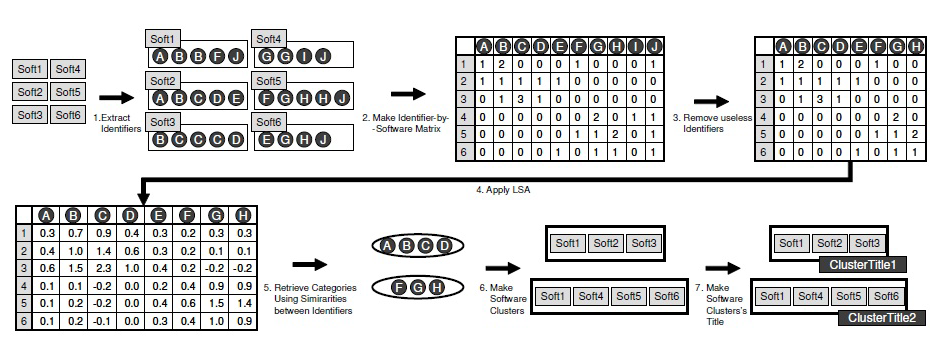
\includegraphics[width=15cm,height=20cm,keepaspectratio]{images/Mudablue1.png}
	\centering
	\caption{The MUDABlue working phases \cite{10.1109/APSEC.2004.69}}
	\label{fig:MUDABlue}
\end{figure}

With the application of Latent Semantic Analysis, software is considered as a document and each identifier is a word. LSA is used for extracting and representing the contextual usage meaning of words by statistical computations applied to a large corpus of text. In summary, the process that \MUDABlue applies is depicted in Figure~\ref{fig:MUDABlue} and consists of the following steps \cite{10.1109/APSEC.2004.69}:% to compute similarities between software systems:

%The MUDABlue approach can be briefly summarized in 7 steps, as the following image depicts:

%\subsection{Extract Identifiers}
%With identifier we are talking about relevant strings that can allow to characterize a document. In this phase each repository is scanned in order to find the target files, and for each of them the identifiers are exctracted, avoiding adding useless items such as comments. The dataset was a 41C projects gathered from SourceForge.
%
%\subsection{Create identifier-by-software matrix}
%As stated before, the main item to work with is the term-document matrix, in this case we count how many times each term appears in each file for all the projects. The result is matrix \textbf{m x n} with m terms and n projects.
%
%\subsection{Remove useless identifiers}
%From the matrix we remove all the useless terms, that is all the terms that apperas in just one repository, considered a specific terms, and all the terms that appears in more than 50\% of the repositories, considered as general terms.
%
%\subsection{Apply the LSA}
%Once the matrix is ready con be worked, the \emph{SVD} procedure is applied and then the LSI. As explained before [NOTE] the \emph{SVD} procedure decompose the original matrix in 3 other matrices. When we multiply back these matrices we use a rank reducted version of the S matrix in order to generete the final one. The authors didn't provide us any details about their final rank value, so we tested many values and eventually selected one.
%
%\subsection{Apply the Cosine Similarity}
%By using the cosine similarity method, we compare each repository vector with all the others and eventually getting an \textbf{n x n} matrix, in which is expressed the similarity of all the repository couple, with a value \emph{[0.0-1.0]}. Thereafter, the cluster analysis is applied using calculated similarities. 
%
%\subsection{Categorization}
%Make software clusters from identifier clusters. From each identifier clusters, the software systems that contain one or more identifiers in the cluster are retrieved. The last step is to make software clusters’ titles. This can be done by summing all identifier-vectors comprised in the identifier cluster and then consider the ten identifiers that got the highest value in the summation vector.


\begin{itemize}
	
	\item[i)] Extracts identifiers from source code and removes unrelated content;
	\item[ii)] Creates an identifier-software matrix with each row corresponds to one identifier and each column corresponds to a software system;%by considering software system as a document and an identifier as a word;
	\item[iii)] Removes unimportant identifiers, i.e. those that are too rare or too popular;
	\item[iv)] Performs LSA on the identifier-software matrix and computes similarity on the reduced matrix using cosine similarity; 
\end{itemize}



MUDABlue has been evaluated on a database consisting of software systems written in C \cite{10.1109/APSEC.2004.69}. The outcomes of the evaluation were compared against two existing approaches, namely GURU \cite{Maarek:1991:IRA:126244.126254}, and the SVM based method by \emph{Ugurel et al} \cite{Ugurel:2002:WCA:775047.775141}. The evaluation shows that MUDABlue outperforms these observed algorithms with regards to precision and recall.


\section{CLAN: Finding Related Applications}\label{sec:clan}

\CLAN (Closely reLated ApplicatioNs) \cite{McMillan:2012:DSS:2337223.2337267} is an approach for automatically detecting similar Java applications by exploiting the semantic layers corresponding to packages class hierarchies. CLAN works based on the document framework for computing similarity, semantic anchors, e.g. those that define the documents' semantic features. Semantic anchors and dependencies help obtain a more precise value for similarity computation between documents. The assumption is that if two applications have API calls implementing requirements described by the same abstraction, then the two applications are more similar than those that do not have common API calls. The approach uses API calls as semantic anchors to compute application similarity since API calls contain precisely defined semantics. The similarity between applications is computed by matching the semantics already expressed in the API calls. The working process applied by \CLAN is shown in Figure~\ref{fig:CLAN}.

%\textit{CLAN} \cite{McMillan:2012:DSS:2337223.2337267} is an approach for automatically detecting similar Java applications by exploiting the semantic layers corresponding to packages class hierarchies. \textit{CLAN} works based on the document framework for computing similarity, semantic anchors, e.g. those that define the documents' semantic features. Semantic anchors and dependencies help obtain a more precise value for similarity computation between documents. The assumption is that if two applications have API calls implementing requirements described by the same abstraction, then the two applications are more similar than those that do not have common API calls. The approach uses API calls as semantic anchors to compute application similarity since API calls contain precisely defined semantics. The similarity between applications is computed by matching the semantics already expressed in the API calls.

%The process consist of 12 steps here graphically reported.

\begin{figure}[!h]
	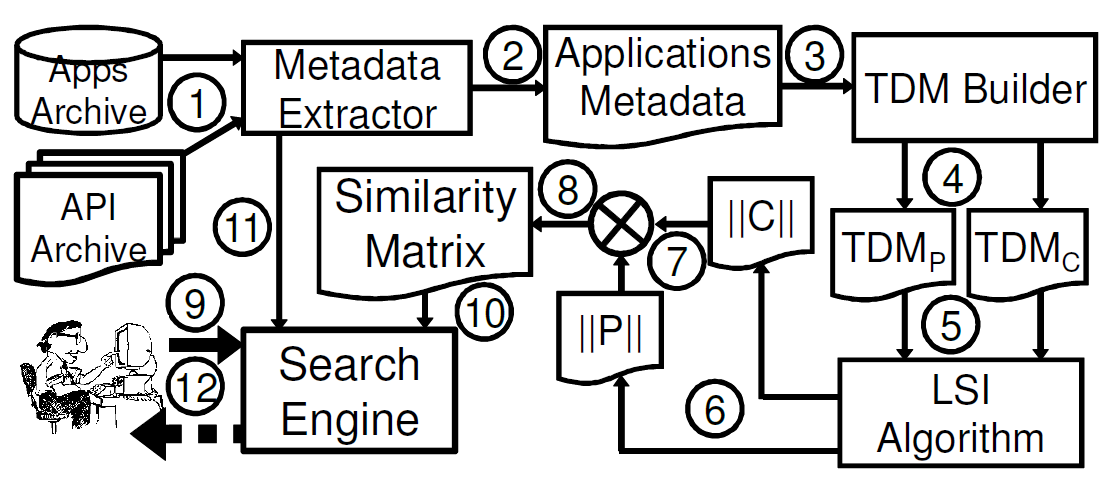
\includegraphics[width=0.80\textwidth]{images/Clan.png}
	\centering
	\caption{The \CLAN working phases \cite{McMillan:2012:DSS:2337223.2337267}}
	\label{fig:CLAN}
\end{figure}

%
%\subsection{Terms Extraction}
%Steps from 1 to 3 can be merged together since are related to extraction of terms from the repositories.
%As stated before, an important concept is that terms extracted are only API calls, this means that all other things present in a piece of code are discarded, for example all the variables or the function declaration and invocation. Furthermore these API calls belong only to the JDK, in such a way also the calls to any other external library are discarded. This idea is also applied in the extraction of the import declaration, focus only on the JDK packages import.
%The result of this process will be an ordered set of data, representing the occurrencies of any Package;Class for all the projects.
%
%\subsection{TDMs Creation}
%Once the dataset as been created, is reorganized in TDMs. Here two different matrices are created, one for the Classes and one for the Packages. Class-level and package-level similarities are different since applications are often more similar on the package level than on the class level because there are fewer packages than classes in the JDK. Therefore, there is the higher probability that two applications may have API calls that are located in the same package but not in the same class.
%
%\subsection{LSI Procedure}
%The paper refers to LSI procedure, Latent Semantic Indexing[dumais2], but the term are synonym, so from here on, we will refer as Latent Semantic Analysis LSA.
%
%\subsection{Apply the Cosine Similarity}
%As for Mudablue, we will apply the cosine similarity to the matrix got from the LSA procedure.
%
%\subsection{Sum of the matrices}
%The 2 matrices are summed, but before are multplied by a certain value. Since the values for the entries in the 2 matrices are between 0.0 and 1.0 a simple sum could result in a value over 1.0, by this multiplication these values are reducted in order to be summed togheter but still maintaining the logical meaning. The authors chosen 0.5, also we, since is a good value to equal distribute the weight of the packages and method calls.The sum of this value is 1.0, and can span from 0.1 to 0.9 for each matrix, is clear that more is high on a matrix, more is important the values that we are considering from such matrix.
%
%\subsection{Final similarity matrix}
%Once the matrix is ready, the system will use it to answer the query of users, from such  matrix the system will retrieve the common projects ordered by rank.



Using a complete software application as input, CLAN represents source code files as a TDM, in which a row contains a unique class or package and a column corresponds to an application. SVD is then applied to reduce the dimension of the matrix. Similarity between applications is computed as the cosine similarity between vector in the reduced matrix. CLAN has been tested on a dataset with more than $8.000$ SourceForge\footnote{SourceForge: \url{https://sourceforge.net/}} applications and shows that it qualifies for the detection of similar applications \cite{McMillan:2012:DSS:2337223.2337267}.

MUDABlue and CLAN are comparable in the way they represent software and source code components like variables, function names or API calls in a term-document matrix and then apply LSA to find the similarity and to category the softwares. However, CLAN has been claimed to help obtain a higher precision than that of MUDABlue as it considers only API calls to represent software systems. 


\section{TagSim: Collaborative Tagging to Detect Similar Applications}\label{sec:tagsim}

In \cite{Lo:2012:DSA:2473496.2473616} tags are leveraged to characterize applications and then to compute similarity between them. Tags are terms that are used to highlight the most important characteristics of software systems \cite{xia:tag:2013} and therefore, they help users narrow down the search scope. Some examples of tags are the category of an app, the license of the system, the programming languages. TagSim\footnote{For the sake of clarity, in this thesis we give a name for the algorithms that have not been named originally} can be used to detect similar applications written in different languages. Based on the assumption that tags capture better the intrinsic features of applications compared to textual descriptions, TagSim extracts tags attached to an application and computes their weights. This information forms the features of a given software system and can be used to distinguish it from others. The technique also differentiates between important tags and unimportant based on their frequency of appearance in the analyzed software systems. The more popular a tag across the applications is, the less important it is and vice versa, i.e. the weight of tag $t$ is $w(t) = \frac{1}{|App(t)|}$ where $App(t)$ is the set of applications that have $t$ as tag. Each application is characterized by a feature vector, $\vec{Tag(a)}$, with each entry corresponds to the weight of a tag the application has. Eventually, the similarity between two applications is computed as the cosine similarity between the two vectors:

\begin{equation}
sim(a_{1},a_{2})= CosineSim(\vec{Tag(a_{1})},\vec{Tag(a_{2})})
%\frac{\sum_{t\in Tag(a_{1})\bigcap Tag(a_{2})}w_{t,a_{1}}\times w_{t,a_{2}}}{\sqrt{\sum_{t\in Tag(a_{1})}(w_{t,a_{1}})^{2} }\times \sqrt{\sum_{t\in Tag(a_{2})}(w_{t,a_{2}})^{2}}} 
\end{equation}

To evaluate TagSim, the authors in \cite{Lo:2012:DSA:2473496.2473616} collected and analyzed more than a hundred thousands of projects. A total of $20$ queries were used to study the performance of the algorithm in comparison with CLAN. The authors also performed a user study to manually analyze the extent to which two applications are similar. Afterwards, success rate, confidence, and precision were used as evaluation metrics. The experimental results show that TagSim helps achieve better performance in comparison to CLAN with a success rate of $80\%$.

Similarly, to help users category a new software object, $TagCombine$ has been proposed in \cite{xia:tag:2013}. $TagCombine$ works using three components: a multi-label ranking component, a similarity based ranking component, and a tag-term based ranking component. In this approach, tags are also used to represent a piece of software as a feature vector, and finally to compute similarity. $TagCombine$ has been evaluated against the approach proposed by \emph{Al-Kofahi et. al.} in \cite{Al-Kofahi:2010:FSA:1912607.1913281} using datasets collected from $2$ popular software information sites, StackOverflow\footnote{StackOverflow: \url{https://stackoverflow.com/}} and Freecode\footnote{Freecode: \url{https://www.freecodecamp.org/}} \cite{xia:tag:2013}. Experiment results show that $TagCombine$ gains a better performance compared to the approach presented in \cite{Al-Kofahi:2010:FSA:1912607.1913281}. 


%achieves recall@5 and recall@10 scores of $0.5964$ and $0.7239$, respectively. For the dataset from Freecode, it achieves recall@5 and recall@10 scores of $0.6391$ and $0.7773$, respectively. 



%For project $p_{i}$, if $G_{i} \bigcap R_{i} > 0$, we say that there is a match. $Recall$ $rate@k$ is the proportion of the number of projects having a match to the number of all test projects. 

% have been collected and analyzed to get input information
%For recommending tags in software information sites, averaging over information sites considered, we improve TagRec proposed by Al-Kofahi et al. by 22.65\% and 14.95\%, and the tag recommendation method proposed by Zangerle et al. by 18.5\% and 7.35\% for recall@5 and recall@10 scores, respectively.
%Similar to TagSim, to compute the similarity between two software objects as to represent the tags of a software as a vector.

%

%===========================================================================================================================

\section{CLANdroid: Detecting Similar Android Applications}\label{sec:clandroid}

Inspired by CLAN, CLANdroid was developed for detecting similar Android applications with the assumption that similar apps share some semantic anchors \cite{10.1109ICPC.2016.7503721}. Nevertheless, in contrast to CLAN, CLANdroid works also when source code is not available as it exploits other high-level information. By extending the scope of semantic anchors for Android apps, starting from APK (Android Package) CLANdroid extracts quintuple features, i.e. identifiers, intents from source code, API calls and sensors from JAR files and user permissions from the \textit{AndroidManifest.xml}\footnote{\url{https://developer.android.com/guide/topics/manifest/manifest-intro.html}} specification. This file is a mandatory component for an Android app and it contains important information about it. For each feature, a feature-Application Matrix is built, resulting in five different matrices. Latent Semantic Indexing is applied to all the matrices to reduce the dimensionality. Afterwards, similarity between a pair of applications is computed as the cosine similarity between their corresponding feature vectors from the matrix. Users can query for similar apps with a given app by specifying which feature is taken into consideration. 

Evaluations have been performed in \cite{10.1109ICPC.2016.7503721} to study which semantic anchors are more effective. The authors also analyze the impact of third-party libraries and obfuscated code when detecting similar apps, since these two factors have been shown to have significant impact on reuse in Android apps and experiments using APKs. The evaluation on a dataset shows that computing similarity based on API helps produce higher recall. According to the experimental results, the feature sensor is ineffective in computing similarity. By comparing with a ground-truth dataset collecting from Google Play, the study suggests the mechanism behind the way Google Play recommends similar apps. % for detecting similar apps

%===========================================================================================================================

\vspace{-.2cm}

\section{SimApp: Detecting Similar Mobile Apps by Online Kernel Learning} \label{sec:SimApp}

With the aim of finding apps with similar semantic requirements, SimApp has been proposed in \cite{Chen:2015:SFD:2684822.2685305}. Unlike other approaches that exploit low-level implementation, e.g. source code, API utilization for similarity calculation, SimApp makes use of high-level metadata collected from apps markets for detecting similar mobile applications. By SimApp, if two apps implement related semantic requirements then they are seen as similar. Each mobile application is modeled by a set of features, so called \emph{modalities}	. The following features are incorporated into similarity computation: \emph{Name}, \emph{Category}, \emph{Developer}, \emph{Description}, \emph{Update}, \emph{Permissions}, \emph{Images}, \emph{Content rating}, \emph{Size} and \emph{Reviews}. For each of these features, a function is derived for each of the features to calculate the similarity between applications.

Given a pair of apps $(a_{i},a_{j})$, a kernel function is defined to compute the similarity for each feature as follows: 

\begin{itemize}
	\item \emph{Name}: It is supposed that two apps are similar if they share common words in their name. A string kernel is exploited to compute the similarity between two app names.
	\item \emph{Category}: Apps in the same category are more similar to each other than to apps in different categories.	
	\item \emph{Developer}: Each developer is characterized by the set of apps that she is involved in and the similarity between two apps is computed using a kernel function of their corresponding developer vectors. 
	\item \emph{Description}: The description text of an app is considered as a document and a kernel function is used to compute the similarity between two description documents of $a_{i}$ and $a_{j}$.
	\item \emph{Update}: Developers use update text to describe the changes they made to the new version of the app. Each update is converted to a fixed length vector. The similarity between $a_{i}$ and $a_{j}$ based on update is computed by using a kernel function similar to the one used for Description. 
	\item \emph{Permission}: For each app, there is a list of permissions specifying which resources on the phone the app can use. A feature vector is used to characterize the permissions of an app and the similarity between $a_{i}$ and $a_{j}$ with regards to permission is computed using a kernel function.      
	\item \emph{Images}: Each app is normally attached with a screenshot image. And SimApp considers two app as similar if they have similar screenshot images. In this way a kernel function is exploited to compute the similarity between two images. 
	\item \emph{Content rating}: Each app has content rating to describe its content and age appropriateness.
	\item \emph{Size}: It is supposed that two apps whose size is considerably different cannot be similar.
	\item \emph{User review}: All user reviews for an app is combined in a document and a similar process for other textual contents is applied to compute the similarity between $a_{i}$ and $a_{j}$.
\end{itemize}

%other features, e.g. images: a function that. For the non-textual components, the following kernels have been defined:

For example, the kernel function for measuring similarity between apps $a_{i}$ and $a_{j}$ with names $s_{i}$ and $s_{j}$ is as follows:

\begin{equation}
K^{name}(a_i,a_j) = \sum_{u_k\in \Sigma^{*}} \phi_{u}(s_{i})\phi_{u}(s_{j})
\end{equation}

This kernel function is also applied to other textual contents, i.e. Name, Description, Update, Reviews to compute similarities among apps with regards to these modalities.

The final similarity score for a pair of apps $(a_{i},a_{j})$ is a linear combination of the multiple kernels with weights. Through the use of a set of training data, the optimal weights are determined by means of online learning techniques. 

\begin{equation}
K(a_{i},a_{j};w)= \sum_{k=1}^n{w_{k}K^k(a_{i},a_{j})}
\end{equation}

%===========================================================================================================================

%\vspace{-.2cm}

\section{AnDarwin: Detecting Similar Android Applications}\label{sec:andarwin}

AnDarwin is an approach that applies Program Dependence Graphs to represent apps \cite{Crussell2013}. Feature vectors are then clustered to find similar apps. Locality Sensitive Hashing is used to find approximate near-neighbors from a large number of vectors. AnDarwin works in the following stages:

\begin{itemize}
	\item[i)] It represents each app as a set of vectors computed over the app's Program Dependence Graphs; %(Section 4.1).
	\item[ii)] Similar code segments are found by clustering all the vectors of all apps;% (Section 4.2).
	\item[iii)] It eliminates library code based on the frequency of the clusters;% (Section 4.3).
	\item[iv)] Finally, it detects apps that are similar, considering both full and partial app similarity.% (Section 4.4).
\end{itemize}

AnDarwin has been applied to find similar apps by different developers (cloned apps) and groups of apps by the same developer with high code reuse (rebranded apps). 

%===========================================================================================================================

%\vspace{-.3cm}

\section{GPLAG: Using Graph for Detecting Software Plagiarism}\label{sec:gplag}

GPLAG is an approach for detecting software plagiarism using program dependence graph \cite{Liu:2006:GDS:1150402.1150522}. Using different input information, GPLAG represents source code files as a graph and detect plagiarism by identifying similar graph patterns. The algorithm captures the control flow and data dependencies between the code statement inside code fragments.

A program dependence graph (PDG) is a labelled, directed graph that uses variable declarations, variable assignments, procedure calls to represent the data and control dependencies within one source code procedure. Code statements are represented by vertices and the dependencies of data and control between statements are edges. A PDG represents the data flow between statements as well as the control between statements. Using the representation, PDG encodes the program logic, thereby representing developers' intention. Given an original program $P_{O}$, and a plagiarism suspect $P_{S}$, plagiarism detection tries to search for duplicate structures. Graph isomorphism is performed to compute the similarity between the PDGs to detect whether two procedures are similar or not. 

%\vspace{-.3cm}

%===========================================================================================================================
\section{WuKong: Detecting Cloned Android Apps}\label{sec:wukong}

WuKong is a proposed approach to detect Android apps clone \cite{Wang:2015:WSA:2771783.2771795}. It is based on a two-phase process which first exploits the frequency of Android API calls to filter out external libraries. Afterwards, a fine-grained phase is performed to compare more features on the set of apps coming from the first phase. For each variable, its feature vector is formed by counting the number of occurrence of variables in different contexts (Counting Environments - CE). An $m$-dimensional Characteristic Vector (CV) is generated using $m$ CEs, where the $i$-th dimension of the CV is the number of occurrences of the variable in the $i$-th CE. For each code segment, CVs for all variables are computed. A code segment is represented by an $n \times m$ Characteristic Matrix (CM). For each app, all code segments are modelled using CM, yielding a series of CMs and they are considered as the features for the app. The similarity between two apps is computed as the proportion of similar code segments. The similarity between two variables $v_{1}$ and $v_{2}$ is computed using cosine similarity between their feature vectors $\vec{V_{1}}$ and $\vec{V_{2}}$:

\begin{equation}
sim(v_{1},v_{2}) = CosineSim(\vec{V_{1}},\vec{V_{2}})%\frac{\sum_{i=1}^{n}a_{i}\cdot b_{i}}{\sqrt{\sum_{i=1}^{n}(a_{i})^{2} }\cdot \sqrt{\sum_{i=1}^{n}(b_{i})^{2}}}
\end{equation}

Evaluations on more than $100,000$ Android apps collected from $5$ Chinese app markets show that the approach can effectively detect cloned apps \cite{Wang:2015:WSA:2771783.2771795}. 

%===========================================================================================================================

\section{LibRec: Automated Library Recommendation}\label{sec:librec}

To help developers leverage existing libraries, LibRec is proposed to provide them with library recommendations \cite{6671293}. LibRec suggests the inclusion of libraries that may be useful for a given project using a combination of rule mining and collaborative filtering techniques. It finds a set of relevant libraries, based on the current set of libraries that a project already uses. Association rule mining is applied to find similar libraries that co-exist in many projects. A collaborative filtering technique is applied to search for top most similar projects and recommends libraries used by these projects to a given project \cite{6671293}.

\begin{itemize}
	%\item Frequent itemset mining:
	\item \textit{Association rule}: the common co-occurrence of libraries in an application. The association rule mining component extracts libraries that are commonly used together. The component then rates each of the libraries based on their likelihood to appear together with the currently used libraries.
	\item \textit{Collaborative Filtering}: Given a project, similarity is computed against all projects and top similar projects are selected. The libraries used by the top similar projects are used as recommendations based on a score computed according to their popularity. 
\end{itemize}

Considering a set of projects $R=(p_{1},p_{2},...p_{m})$ and a set of libraries $L=(l_{1},l_{2},...l_{n})$, each project is characterized by a feature vector using the set of libraries it includes, i.e. $\vec{P_{i}}=(I_{i}(l_{1}),I_{i}(l_{2}),..I_{i}(l_{n}))$, where $I_{i}(l_{r})$ is the inclusion of library $l_{r}$ in project $p_{i}$. $I_{i}(l_{r})=1$ if $l_{r}$ is used in $p_{i}$, otherwise $I_{i}(l_{r})=0$. The similarity between two projects is the cosine similarity between their feature vectors as follows:


\begin{equation}
sim(p_{i},p_{j})=CosineSim(\vec{P_{i}},\vec{P_{j}})
%\frac{\sum_{r=1}^{n} I_{i}(l_{r}) \times I_{j}(l_{r}) }{\sqrt{\sum_{r=1}^{n} I_{i}(l_{r})^{2} }\times \sqrt{\sum_{r=1}^{n}I_{j}(l_{r})^{2}}} 
\end{equation}


Ten-fold cross validation is applied on a dataset of $500$ GitHub projects that use at least $10$ third-party libraries to evaluate the performance of LibRec \cite{6671293}. The dataset is divided into $10$ equal parts, so-called \emph{sub-samples}. The validation was conducted for ten times and for each time, nine sub-samples are used as training data and the remaining sub-sample is used as test data. For each testing project, a half of its libraries is taken out and used as ground-truth data and the other half is used to compute the similarities to all projects in the training set to get library recommendation. The experiments show that the libraries recommended by LibRec match the ones that are already stored in the ground-truth data with high recall rate.


\section{RepoPal: A tool to detect similar GitHub projects} \label{sec:repopal}

In contrast to many previous studies that are generally based on source code \cite{10.1109/APSEC.2004.69},\cite{Liu:2006:GDS:1150402.1150522},\cite{McMillan:2012:DSS:2337223.2337267}, RepoPal  \cite{10.1109/SANER.2017.7884605} is a high-level similarity metric and takes only repositories metadata as its input. With this approach, two GitHub\footnote{About GitHub: \url{https://github.com/about}} repositories are considered to be similar if:

\begin{itemize}
	\item[i)] They contain similar \code{README.MD} files;
	\item[ii)] They are starred by users of similar interests;
	\item[iii)] They are starred together by the same users within a short period of time. 
\end{itemize}

Thus, the similarities between GitHub repositories are computed by using three inputs: readme file, stars and the time gap that a user stars two repositories. Considering two repositories $ r_{i} $ and $ r_{j} $, the following notations are defined: 

\begin{itemize}
	\item $ f_{i} $ and $ f_{j} $ are the readme files with $ t $ being the set of terms in the files; 
	\item $ U(r_{i}) $ and $ U(r_{j}) $ are the set of users who starred $ r_{i} $ and $ r_{j} $, respectively; 
	\item $ R(u_{k}) $ is the set of repositories that user $ u_{k} $ already starred.  
\end{itemize}

There are three similarity indices as follows:

\paragraph{Readme-based similarity} 

The similarity between two readme files is calculated as the cosine similarity between their feature vectors $\vec{f_{i}}$ and $\vec{f_{j}}$: 

\begin{equation}
sim_{f}(r_{i},r_{j})=CosineSim(\vec{f_{i}},\vec{f_{j}})
\end{equation}

%\frac{\sum_{t\in f_{i}\bigcap f_{j}}w_{t,f_{i}}\times w_{t,f_{j}}}{\sqrt{\sum_{t\in f_{i}}(w_{t,f_{i}})^{2} }\times \sqrt{\sum_{t\in f_{j}}(w_{t,f_{j}})^{2}}} 

\paragraph{Stargazer-based similarity}

The similarity between a pair of users $ u_{k} $ and $ u_{l} $ is defined as the Jaccard index \cite{jaccard} of the sets of repositories that $ u_{k} $ and $ u_{l} $ have already starred:% (Section \ref{sec:jaccard})

\begin{equation} \label{eqn:StarBasedSim}
sim_{u}(u_{k},u_{l})=Jaccard(R(u_{k}),R(u_{l}))
%\frac{|R(u_{k})\bigcap R(u_{l})|}{|R(u_{k})\bigcup R(u_{l})|} 
\end{equation}

The star-based similarity between two repositories $ r_{i} $ and $ r_{j} $ is the average similarity score of all pairs of users who already starred $ r_{i} $ and $ r_{j} $:% as follows

\begin{equation} %\label{eqn:StarBasedSim}
sim_{s}(r_i,r_j) = \frac{1}{|U(r_{i})|\cdot |U(r_{j})|}\sum_{\substack{u_k\in U(r_i)\\
		u_l\in U(r_j)}}sim_{u}(u_k,u_l)\\
\end{equation}


\paragraph{Time-based similarity} It is supposed that if a user stars two repositories during a relative short period of time, then the two repositories are considered to be similar. Based on this assumption, given that $T(u_{k},r_{i},r_{j})$ is the time gap that user $u_{k}$ stars repositories $r_{i}$ and $r_{j}$, the time-based similarity is computed as follows:%the average period of time that lapsed between the time the two repositories were starred by each person.


\begin{equation} %\label{eqn:TimeBasedSim}
sim_{t}(r_i,r_j) = \frac{1}{|U(r_{i}) \cap U(r_{j})|}\sum_{u_k\in U(r_{i}) \cap U(r_{j})}\frac{1}{|T(u_k,r_i,r_j)|}
\end{equation}

%According to the authors, the time-based similarity has been added to filter out the results t

Finally, the similarity between two projects is the product of the three similarity indices: % combination of the three similarity indices using multiplication:

\begin{equation} \label{eqn:RepoPalSim}
sim(r_i,r_j) = sim_{f}(r_i,r_j) \times sim_{s}(r_i,r_j) \times sim_{t}(r_i,r_j)
\end{equation}

RepoPal has been evaluated against CLAN using a dataset of $1,000$ Java repositories \cite{10.1109/SANER.2017.7884605}. Among them, $50$ were chosen as queries. {\em Success Rate}, {\em Confidence} and {\em Precision} were used as the evaluation metrics. Experimental results in the paper show that RepoPal produces better quality metrics than those of CLAN.


%In summary, by reviewing other additional similarity metrics \cite{Crussell2013,10.1109ICPC.2016.7503721,Liu:2006:GDS:1150402.1150522,xia:tag:2013} which cannot be presented here due to space limitation, we have seen that they normally deal with either low-level or high-level similarity. 

%In, we introduce a preliminary version of this work on CrossSim \cite{NDRDSEAA2018}. In \cite{DBLP:conf/iir/NDD013} a graph structure has been exploited to recommend third-party libraries.




\section{\CrossSim: Detecting similar OSS projects using graph}

In recent years, considerable effort has been made to provide automated assistance to developers in navigating large information spaces and giving recommendations. Though remarkable progress can be seen in this field, there is still room for improvement. To the best of our knowledge, most of the existing approaches consider the constituent components of the OSS ecosystem separately, without paying much attention to their mutual connections. There is a lack of a proper scheme that facilitates a unified consideration of various OSS artifacts and recommendations. \CrossSim \cite{NDRDSEAA2018},\cite{NDD:KaRS:2018},\cite{DBLP:conf/iir/NDD013} has been proposed as a novel approach to compute similarity.
 
 \begin{figure}[!h]
 	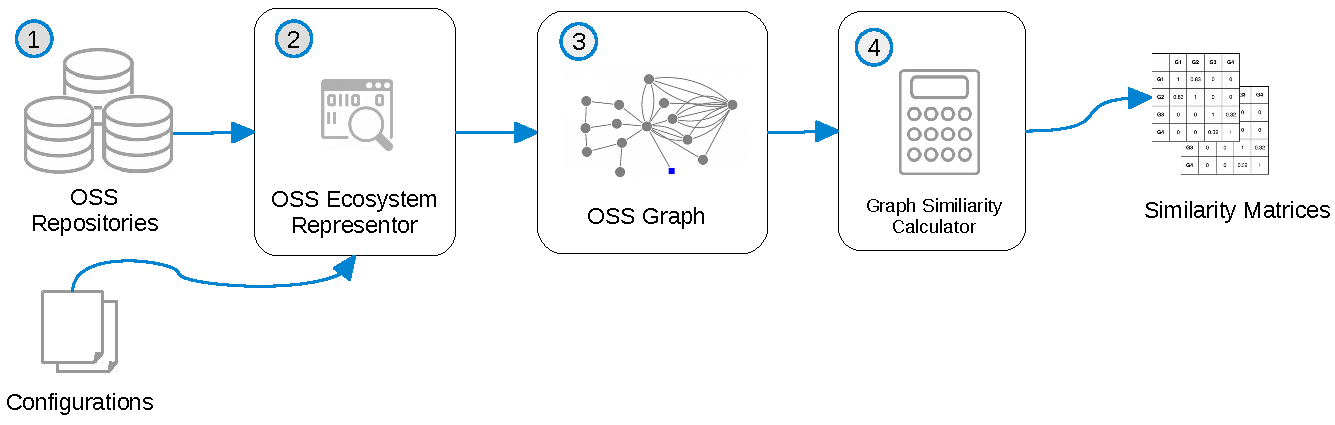
\includegraphics[width=15cm,height=20cm,keepaspectratio]{images/CrossSim.pdf}
 	\caption{The \CrossSim Architecture}
 	\label{fig:CrossSim}
 \end{figure}
 
The architecture of CrossSim is depicted in Figure \ref{fig:CrossSim}: the rectangles represent artifacts, whereas the ovals represent activities that are automatically performed by the developed CrossSim tooling. In particular, the approach imports project data from existing OSS repositories and represents them into a graph-based representation by means of the \emph{OSS Ecosystem Representation} module. Depending on the considered repository (and thus to the information that is available for each project) the graph structure to be generated has to be properly configured. For instance in case of GitHub, specific configurations have to be specified in order to enable the representation in the target graphs of the stars assigned to each project. Such a configuration is ``forge'' specific and specified once, e.g., SourceForge does not provide the star based system available in GitHub. 
 %
The \emph{Graph similarity} module implements the SimRank algorithm \cite{Jeh:2002:SMS:775047.775126} that is applied on the source graph-based representation of the input ecosystems generates matrices representing the similarity value for each pair of input projects. 
 
% \subsection{Graph-based Representation of OSS Ecosystems}
 
We consider the community of developers together with OSS projects, libraries and their mutual interactions as an \emph{ecosystem}. In this system, either humans or non-human factors have mutual dependency and implication on the others. There, several connections and interactions prevail, such as developers commit to repositories, users star repositories, or projects contain source code files, just to name a few. We propose a solution that makes use of graphs for representing relationships in OSS ecosystems. Specifically, the graph model has been chosen since it allows for flexible data integration and facilitates numerous similarity metrics and clustering techniques \cite{Blondel:2004:MSG:1035533.1035557},\cite{Lu2007},\cite{Schaeffer:2007:SGC:2296006.2296057}. All the playing actors and their communications are transformed into a directed graph. Humans and non-human artifacts are represented as nodes and there is a directed edge between a pair of nodes if they interact with each others. The representation model considers different artifacts in a united fashion, taking into account their mutual, both direct and indirect relationships as well as their co-occurrence as a whole. The representation is twofold: First, it incorporates semantic relationships into the graph. Second, it helps combine both low-level and high-level information into a homogeneous representation.
 
 
 
 \begin{figure}[t!]
 	\centering
 	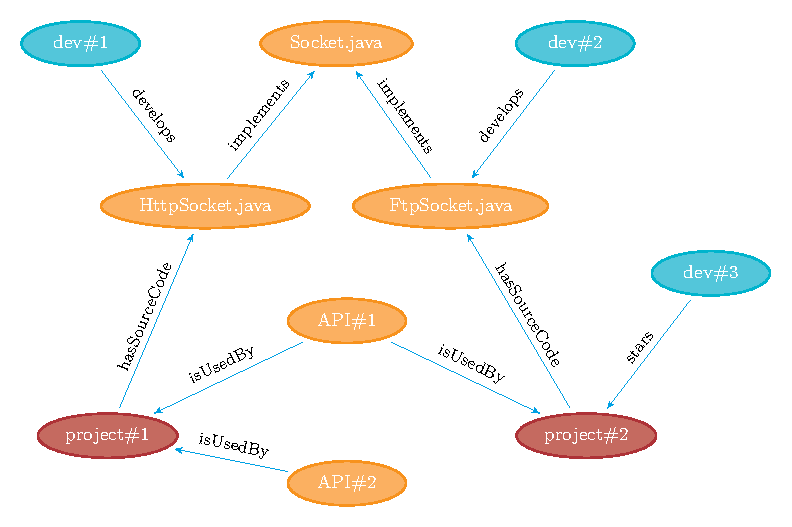
\includegraphics[width=0.60\textwidth]{images/OSSGraph1.pdf}
 	\caption{Sample graph-based representation of OSS ecosystems}
 	\label{fig:OSSGraph1}
 \end{figure}
 
 
To demonstrate the utilization of graphs in an OSS ecosystem, we consider an excerpt of the dependencies for two OSS projects, namely \texttt{project\#1} and \texttt{project\#2} in Figure~\ref{fig:OSSGraph1}. Using dependency information extracted from source code and the corresponding metadata (e.g. coming from the tools developed in by Work Package 2), this graph can be properly built to represent the two projects as a whole. In this figure, \texttt{project\#1} contains code file \texttt{HttpSocket.java} and \texttt{project\#2} contains \texttt{FtpSocket.java} with the corresponding edges being marked with the semantic predicate \texttt{hasSourceCode}. Both source code files implement \texttt{interface\#1} being marked by the semantic predicate \texttt{implements}. \texttt{Project\#1} and \texttt{project\#2} are also connected via other semantic paths, such as API \texttt{isUsedBy} highlighted in Figure~\ref{fig:OSSGraph3}. In practice, an OSS graph is much larger with numerous nodes and edges, and the relationship between two projects can be thought as a sub-graph. 
 
 \begin{figure}[h!]
 	\centering
 	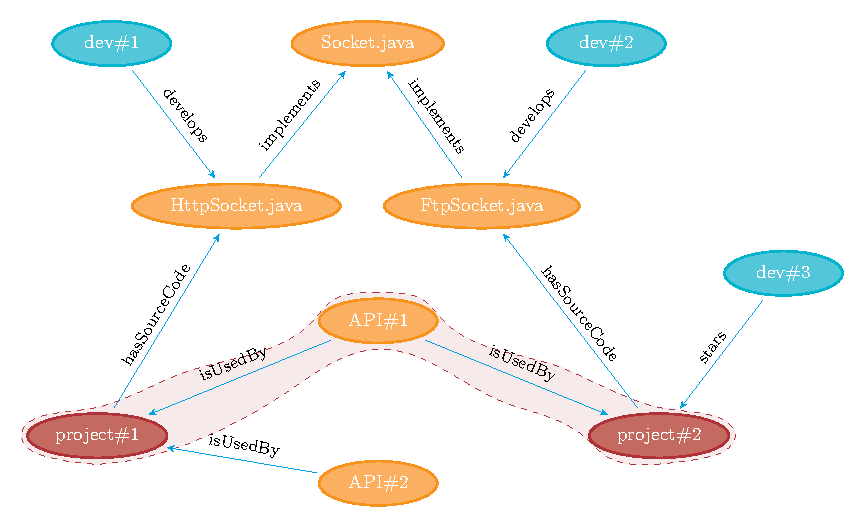
\includegraphics[width=0.60\textwidth]{images/OSSGraph3.pdf}
 	\caption{Similarity between OSS projects with respect to API usage}
 	\label{fig:OSSGraph3}
 \end{figure}
 
 
Based on the graph structure, one can exploit nodes, links and the mutual relationships to compute similarity using existing graph similarity algorithms. To the best of our knowledge, there exist several metrics for computing similarity in graph \cite{Blondel:2004:MSG:1035533.1035557},\cite{Nguyen:2015:CRV:2942298.2942305},\cite{Nguyen:2015:ESP:2740908.2742141}. The graph structure also allows for graph kernel methods, which are an effective way to compute similarity \cite{ODMD14a}. Considering Figure~\ref{fig:OSSGraph1}, we can compute the similarity between \texttt{project\#1} and \texttt{project\#2} with regards to the semantic paths between them, e.g. the two-hop path using \texttt{hasSourceCode} and \texttt{implements} (Figure~\ref{fig:OSSGraph2}), or the one-hop path using API \texttt{isUsedBy}. For example, concerning \texttt{isUsedBy}, the two projects are considered to be similar since with the predicate both projects originate from \texttt{API\#1}. The hypothesis is based on the fact that the projects are aiming at creating common functionalities by using common libraries \cite{McMillan:2012:DSS:2337223.2337267},\cite{6671293}.
 
 
 \begin{figure}[h!]
 	\centering
 	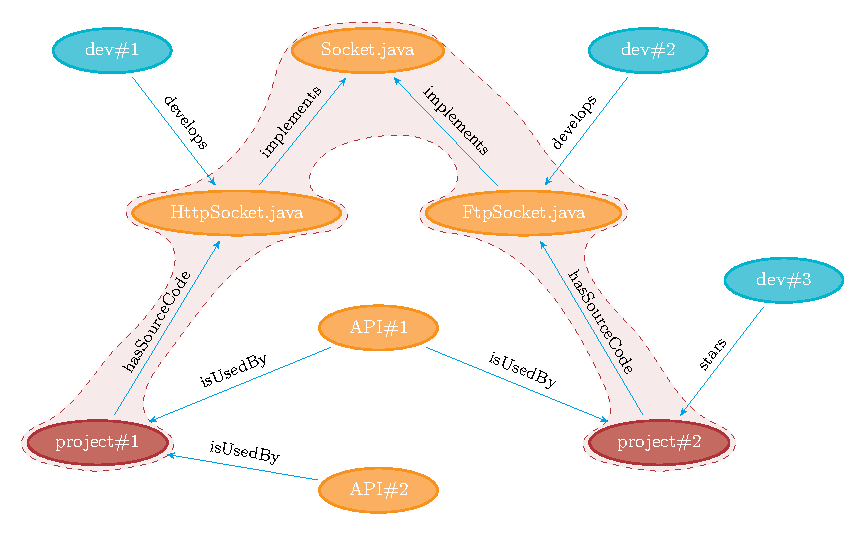
\includegraphics[width=0.60\textwidth]{images/OSSGraph2.pdf}
 	\caption{Similarity between OSS projects with respect to source implementation}
 	\label{fig:OSSGraph2}
 \end{figure}
 
 
The representation allows us to compute similarity between other graph components, e.g. developers. Back to Figure~\ref{fig:OSSGraph1}, though there is no direct connection between \texttt{dev\#1} and \texttt{dev\#2}, their similarity can still be inferred from indirect semantic paths, such as \texttt{develops} and \texttt{implements} which are highlighted in Figure \ref{fig:OSSGraph4}.
 %
If we consider other semantic paths, we see that the two developers have more in common as they both take part in \texttt{project\#1} and \texttt{projects\#2} represented by \texttt{commits}. To a certain extent, the two developers are considered to be similar, although they are not directly connected. In reality, the connection between \texttt{developer\#1} and \texttt{developer\#2} is enforced by further semantic paths and as a result their similarity can be more precisely computed. The similarities between developers can serve as input for a collaborative filtering recommendation system, with which a developer is recommended a list of projects or libraries that similar developers already worked with \cite{Pazzani2007},\cite{Schafer:2007:CFR:1768197.1768208}. This is an invaluable tool in the context of the \projectName project since it is essential to equip developers with recommendation functionalities to help them increase reusability and productivity.
 
 
% \begin{figure}[t!]
% 	\centering
% 	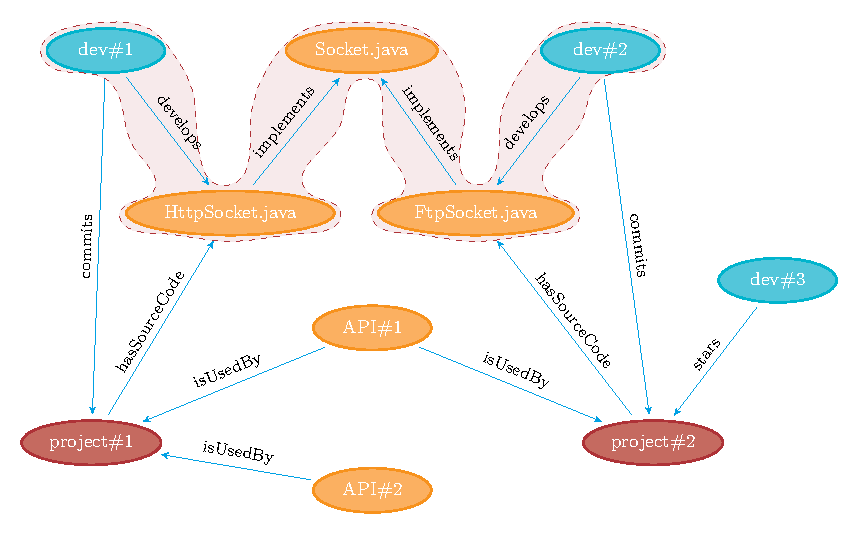
\includegraphics[width=0.60\textwidth]{images/OSSGraph4.pdf}
% 	\caption{Similarity between developers}
% 	\label{fig:OSSGraph4}
% \end{figure}

%\clearpage
 
 
The relationships underpinning the graph-based representations of the simple ecosystems shown in Fig. \ref{fig:OSSGraph1}--\ref{fig:OSSGraph3} are shown in Table~\ref{tab:Representation}. For the first implementation of \CrossSim the relationships $isUsedBy$, $develops$, and $stars$ have been considered. 
 
 
 \begin{table}[h!]
 	\centering
 	\begin{tabular}{|p{5.4cm}|p{8cm}|}  \hline
 		{\bf Relationship} & {\bf Description} \\  \hline
 		\textit{isUsedBy} $\subseteq$ \textit{Dependency}$\times$\textit{Project} & this relationship depicts the reliance of a project on a dependency (e.g., a third-party library). The project needs to include the dependency in order to function. According to \cite{McMillan:2012:DSS:2337223.2337267,6671293} the similarity between two considered projects relies on the dependencies they have in common because they aim at implementing similar functionalities.\\ \hline
 		\textit{develops} $\subseteq$ \textit{Developer} $\times$ \textit{Project} & we suppose that there is a certain level of similarity between two projects if they are built by same developers, as already hypothesized by \cite{Chen:2015:SFD:2684822.2685305}. Thus, this relationship is used to represent the projects that a given user contributes in terms of source code development.\\ \hline
 		\textit{stars} $\subseteq$ \textit{User} $\times$ \textit{Project} & This relationship is inspired by the star event in RepoPal \cite{10.1109/SANER.2017.7884605} to represent GitHub projects that a given user has starred. However, we consider the star event in a broader scope in the sense that not only direct but also indirect connections between two developers is taken into account.\\ \hline
 		\textit{implements} $\subseteq$ \textit{File} $\times$ \textit{File} & It represents a specific relation that can occur between the source code given in two different files, e.g. a class specified in one file implementing an interface given in another file.	\\ \hline
 		\textit{hasSourceCode}  $\subseteq$ \textit{Project} $\times$ \textit{File} & It represents the source files contained in a given project.\\\hline
 	\end{tabular}
 	\caption[Relationships]{Graph Representation of OSS projects}
 	\label{tab:Representation}
 \end{table}
 
%\subsection{Similarity Computation}









\section{Analysis} \label{sec:Analysis}

In this section we present a review on the above mentioned similarity metrics. The review is twofold as follows. First, it helps determine the features that contribute effectively towards similarity computation in OSS projects. Second, it aims at evaluating and identifying the strength as well as the shortcomings of the approaches. Table~\ref{tbl:AlgorithmsAndFeatures} shows a summary of the previously outlined approaches with respect to the features, which are exploited by each technique. In particular, the features shown in Table~\ref{tbl:AlgorithmsAndFeatures}  are:

\begin{itemize}
	\item {\em LOC}: the number of lines of code.
	\item {\em Dep.}: the third-party libraries a project includes.
	\item {\em API calls}: API function calls appear in source code. They are used to build term-document matrices and then to calculate similarities among applications.
	%\item {\em Library}: Third-party libraries used.
	\item {\em Function}: functions and procedures defined in the source code.
	\item {\em Star}: star events in GitHub. Different from the concept of stars or bubbles used in other rating systems like TripAdvisor\footnote{\url{https://www.tripadvisor.com/TripAdvisorInsights/n2640/all-about-your-tripadvisor-bubble-rating}} or Facebook\footnote{\url{https://www.facebook.com/help/548274415377576/}}, stars in GitHub are not used to rate a repository. A developer stars a repository as a way to keep track of it for future reference. In addition, stars are used as a means to thank the repository maintainers for their contribution\footnote{\url{https://help.github.com/articles/about-stars}}.
	\item {\em Timestamp}: the point of time when a user stars a repository. %This feature is used only by RepoPal \cite{10.1109/SANER.2017.7884605}.
	\item {\em Statement}: source code statement.
	\item {\em Readme}: Readme.md or description file, used to describe the functionalities of an open source project. 
	\item {\em Tag}: tags are used by OSS platforms, e.g. SourceForge to classify and characterize an open source project.
	\item {\em Update}: the newest changes made to the app.
	\item {\em Permission}: this feature is available only by mobile apps. It specifies the permission of an app to handle data in a smartphone.
	\item {\em Screenshot}: this feature is available by mobile apps. It is used to compare different apps.
\end{itemize}

As shown in Table~\ref{tbl:AlgorithmsAndFeatures} the techniques that mainly underpin the outlined similarity approaches are:

\begin{itemize}
	\item {\em TDM \& LSA}: Term-Document Matrix \cite{Collobert:2011:NLP:1953048.2078186} and Latent Semantic Analysis \cite{Landauer1998} are generally used in combination to model the relationships between API calls/identifiers and software systems and to compute the similarities between them.
	\item {\em COS}: Cosine Similarity, this technique is widely used in several algorithms for computing similarities among vectors.
	\item {\em JCS}: Jaccard index used for computing similarity between two sets of elements~\cite{jaccard}.
\end{itemize}


Most low-level similarity algorithms (shown as \textit{L} in Table~\ref{tbl:AlgorithmsAndFeatures}) attempt to represent source code (and API calls) in a term-document matrix and then apply SVD to reduce dimensionality. The similarity is then computed as the cosine similarity between feature vectors. Among others, MUDABlue \cite{10.1109/APSEC.2004.69}, CLAN \cite{McMillan:2012:DSS:2337223.2337267}, and CLANdroid \cite{10.1109ICPC.2016.7503721} belong to this category. CLAN includes API calls for computing similarity, whereas, by MUDABlue, every word appearing in source code files is integrated into the term-document matrix. This makes the difference in the performance of the two algorithms in a way that the similarity scores of CLAN reflect better the perception of humans of similarity than those of MUDABlue. %The different 



\begin{landscape}
	\begin{table}[htbp]
		\footnotesize
%		\small
		\centering
		\begin{tabular}{|p{2.5cm}|c|c|c|c|c|c|c|c|c|c|c|}  
			\hline 
			& \textbf{MUDABlue} & \textbf{CLAN} & \textbf{CLANdroid} & \textbf{GPLAG} & \textbf{LibRec} & \textbf{SimApp} & \textbf{AnDarwin} & \textbf{WuKong} & \textbf{TagSim} & \textbf{RepoPal} & \textbf{CrossSim} \\\hline			
			References & \cite{10.1109/APSEC.2004.69} & \cite{McMillan:2012:DSS:2337223.2337267} & \cite{10.1109ICPC.2016.7503721} & \cite{Liu:2006:GDS:1150402.1150522} & \cite{6671293} & \cite{Chen:2015:SFD:2684822.2685305} & \cite{Crussell2013} &  \cite{Wang:2015:WSA:2771783.2771795} & \cite{Lo:2012:DSA:2473496.2473616} & \cite{10.1109/SANER.2017.7884605} & \cite{NDRDSEAA2018} \\\hline
			\multicolumn{12}{|c|}{\bf Features (Modalities)}  \\ \cline{1-12}
			$LOC$ &  &  &  & $\times$ &  &  &  &  &  & &   $\times$ \\\hline
			$Dep.$ &  & $\times$ &  &  &  &  &  &  &  &  & $\times$ \\\hline
			$API$ $Calls$ &  & $\times$ & $\times$ &  & $\times$ &  &  & $\times$ &  & &  $\times$ \\\hline
			$Function$ &  &  &  & $\times$ &  &  &  &  &  &  &  $\times$ \\\hline
			$Star$ &  &  &  &  &  &  &  &   &  & $\times$ &  $\times$ \\\hline
			$Timestamp$ &  &  &  &  &  &  &  &  &   & $\times$  & \\\hline
			$Statement$ & $\times$ &  &  & $\times$ &  &  &  &  &  &   & \\\hline
			$Identifier$  & $\times$ &  & $\times$ &  &  &  &  &  &   &  & \\\hline
			$App. Name$ &  &  &  &  &  & $\times$ &  &  &  & & \\\hline
			$Topic$ &  &  &  &  &  & $\times$ &  &  &  &  & \\\hline
			$Developer$ &  &  &  &  &  & $\times$ &  &  &  &  &  $\times$ \\\hline
			$Readme.md$ &  &  &  &  & $\times$ &  & $\times$ &  & $\times$ & $\times$  & \\\hline
			$Tag$ &  &  &  &  &  &  &  &  & $\times$ &  & \\\hline
			$Update$ &  &  &  &  &  & $\times$ &  &  &   &  & \\\hline
			$Permissons$ &  &  & $\times$ &  &  & $\times$ &  &  &  &  &  \\\hline
			$Screenshot$ &  &  &  &  &  & $\times$ &  &  &  &   & \\\hline
			$Content$ &  &  &  &  &  & $\times$ &  &  &  &  & \\\hline
			$Size$ &  &  &  &  &  & $\times$ &  &  &  &   & \\\hline
			$Reviews$ &  &  &  &  &  & $\times$ &  &  &  & & \\\hline
			$Intent$ &  &  & $\times$ &  &  &  &  &   &   & & \\\hline
			$Sensors$ &  &  & $\times$ &  &  &  &  &  &   & & \\\hline
			
			\multicolumn{12}{|c|}{\bf Used Techniques} \\ \cline{1-12}
			$TDM \& LSA$ & $\times$ & $\times$ & $\times$ &  &  &  &  &  &   &  & \\\hline
			%$LSA$ & $\times$ & $\times$ & $\times$ &  &  &  &  &  &   &  \\ \hline
			$COS$ & $\times$ & $\times$ & $\times$ &  & $\times$ & $\times$ &  & $\times$  &  $\times$ & $\times$  & \\\hline
			$JCS$ &  &  &  &  &  &  & $\times$ &  &  & $\times$ & \\\hline
			
			\multicolumn{12}{|c|}{\bf Category}  \\ \cline{1-12}
			$High/Low$ $Sim$ & L & L & L & L & L & H & H & L & H  & H  & L \& H \\\hline
			
		\end{tabular}
		\caption{Summary of the similarity algorithms and their features}
		\label{tbl:AlgorithmsAndFeatures}
	\end{table}	
\end{landscape}


In contrast, high-level similarity techniques (shown as \textit{H} in Table~\ref{tbl:AlgorithmsAndFeatures}) do not consider source code for similarity computation. They characterize software by exploiting available features such as descriptions, user reviews, and \code{README.MD} file. The similarity is computed as the cosine similarity of the corresponding feature vectors. For computing similarity between mobile applications, other specific features such as images and permissions are also incorporated. A current trend in these techniques is to exploit textual content to compute similarity, e.g. in AppRec \cite{confairsBhandariSDJ13}, SimApp \cite{Chen:2015:SFD:2684822.2685305}, TagSim \cite{Lo:2012:DSA:2473496.2473616}. A main drawback with this approach is that, same words can be used to explain different requirements or the other way around, the same requirements can be described using different words \cite{10.1109/APSEC.2004.69}. So it might be the case that two textual contents with different vocabularies still have a similar description or two files with similar vocabularies contain different descriptions. The matching of words in the descriptions as well as source code to compute similarity is considered to be ineffective as already stated in \cite{McMillan:2012:DSS:2337223.2337267}. To overcome this problem, the application of a synonym dictionary like WordNet \cite{Miller:1995:WLD:219717.219748} is beneficial. Furthermore, the utilization TDM and LSA in textual contents is proven to be effective as LSA helps consider latent semantic relationships. Nevertheless, there is still a problem with the approaches like RepoPal where readme file is used for similarity computation, since in general the descriptions for software projects are written in different languages. According to our observation in GitHub, \code{README.MD} files are written in various languages, \eg not only English but also Japanese, Korean, or Chinese. And the comparison of a readme file in Japanese with one in English should yield dissimilarity, even though two projects may be similar. SimApp \cite{Chen:2015:SFD:2684822.2685305} is the only technique that attempts to combine several high-level information into similarity computation. It eventually applies a machine learning algorithm to learn optimal weights. The approach is promising, nevertheless it is only applicable in the presence of a decent training dataset, which is hard to come by in practice.

\CrossSim is an approach that attempts to combine both low-level and high-level information in computing similarities. The approach integrates implicit semantic relationships and intrinsic dependencies among different users, repositories, source code. Thus, it is able to incorporate new features, on the fly, into the similarity computation without modifying the internal design. \CrossSim is expected to improve the overall performance of the similarity computation and thus the quality of the eventual recommendations. In the next chapters, we are going to introduce our implementation and evaluation of \CrossSim with respect to some notable tools, \ie \MUDABlue, \CLAN, and \RepoPal.


%We aim to design a representation model that integrates semantic relationships among various artifacts and
% By considering all artifacts in a mutual relationship, we aim at improving the overall performance of the similarity computation and
% In the next section, we propose a similarity model that attempts to exploit effectively the rich metadata infrastructure provided by the \projectName Knowledge Base by trying to incorporate various features in computing similarity. Afterwards, we present an initial evaluation on a real dataset collected from GitHub to demonstrate the performance of our approach. 
%in computing similarities and this seems to be beneficial to the context of OSS repositories. 
%should be highly beneficial to the context of OSS repositories. various input information, We hypothesize that combining 
%%==================================Highlight the difference that CrossSim can make, the flexibility==================================
%Most approaches are either low-level or high-level similarity. We see that either a low-level or a high-level similarity metric is able to deal with a certain set of features, they cannot work given that more features are available for similarity computation. In this sense, these metrics can only be applied in a limited context. They can be applied in a limited context, whereas CrossSim gives more flexibility. An approach that is more flexible and overcomes the limitations. The flexibility of. 

%In the next section, we present a novel approach for computing software similarities by allowing one to incorporate various features into the computation.






















%In summary, by reviewing other additional similarity metrics \cite{Crussell2013,10.1109ICPC.2016.7503721,Liu:2006:GDS:1150402.1150522,xia:tag:2013} which cannot be presented here due to space limitation, we have seen that they normally deal with either low-level or high-level similarity. % and to pave the way for . 
%We are convinced that combining various input information in computing similarities is highly beneficial to the context of OSS repositories. We aim to design a representation model that integrates semantic relationships among various artifacts and the model is expected to improve the overall performance of the similarity computation.% and to pave the way for . 


%$SimApp$ \cite{Chen:2015:SFD:2684822.2685305} is the only technique that attempts to combine several high-level information into similarity computation. The approach is promising, nevertheless it is only applicable in the presence of a decent training dataset, which is hard to come by in practice. 
%
%
%\section{A Comprehensive Analysis on the Similarity Metrics} \label{sec:Analysis}
%
%In this section we present a review on the above mentioned similarity metrics. The review is twofold as follows. First, it aims at evaluating and identifying the strength as well as the shortcomings of the approaches. Second, it helps determine the features that contribute effectively towards similarity computation in OSS projects.
%
%Most low-level similarity algorithms attempt to represent source code, API calls in a term-document matrix and then apply SVD to reduce dimensionality. The similarity is then computed as the cosine similarity between feature vectors. Among others, $MUDABlue$ \cite{10.1109/APSEC.2004.69}, $CLAN$ \cite{McMillan:2012:DSS:2337223.2337267}, and $CLANdroid$ \cite{10.1109ICPC.2016.7503721} belong to this category. $CLAN$ includes API calls for computing similarity, whereas, by $MUDABlue$, every word appearing in source code files is integrated into the term-document matrix. This makes the difference in the performance of the two algorithms in a way that the similarity scores of $CLAN$ reflect better the perception of humans of similarity than those of $MUDABlue$. %The different 
%
%In contrast, high-level similarity techniques do not consider source code for similarity computation. They characterize software by exploiting available features such as descriptions, user reviews, readme file. The similarity is computed as the cosine similarity of the corresponding feature vectors. For computing similarity between mobile applications, other specific features such as images and permissions are also incorporated. A current trend in these techniques is to exploit textual content to compute similarity, e.g. in $AppRec$ \cite{confairsBhandariSDJ13}, $SimApp$ \cite{Chen:2015:SFD:2684822.2685305}, $TagSim$ \cite{Lo:2012:DSA:2473496.2473616}. A main drawback with this approach is that, same words can be used to explain different requirements or the other way around, the same requirements can be described using different words \cite{10.1109/APSEC.2004.69}. So it might be the case that two textual contents with different vocabularies still have a similar description or two files with similar vocabularies contain different descriptions. The matching of words in the descriptions as well as source code to compute similarity is considered to be ineffective as already stated in \cite{McMillan:2012:DSS:2337223.2337267}. To overcome this problem, the application of a synonym dictionary like WordNet \cite{Miller:1995:WLD:219717.219748} is beneficial. Furthermore, the utilization TDM and LSA in textual contents is proven to be effective as LSA helps consider latent semantic relationships. Nevertheless, there is still a problem with the approaches like $RepoPal$ where readme file is used for similarity computation, since in general the descriptions for software projects are written in different languages. According to our investigations on GitHub, projects include \emph{readme.md} in various languages, such as Japanese, Korean, and Chinese. And the comparison of a readme file in Japanese with one in English should yield dissimilarity. $SimApp$ \cite{Chen:2015:SFD:2684822.2685305} is the only technique that attempts to combine several high-level information into similarity computation. It eventually applies a machine learning algorithm to learn optimal weights. The approach is promising, nevertheless it is only applicable in the presence of a decent training dataset, which is hard to come by in practice.
%
%We are convinced that combining both low-level and high-level information in computing similarities should be highly beneficial to the context of OSS repositories. We expect a representation model that integrates implicit semantic relationships and intrinsic dependencies among different users, repositories, source code. By considering all artifacts in a mutual relationship, we aim at improving the overall performance of the similarity computation. In the next section, we propose a similarity model that attempts to exploit effectively the rich metadata infrastructure provided by \projectName Knowledge Base by trying to incorporate various features in computing similarity. Afterwards, we present an initial evaluation on a real dataset collected from GitHub to demonstrate the performance of our approach. Apart from $RepoPal$, some additional similarity metrics are derived and work as baselines for comparison. 
%



